	
%%%%%%%%%%%%%%%%%%%%%%%%%%%%%%%%%%%%%%%%%%%%%%%%%%%%%%%%%%%%%%%%%%%%%%%%%%%%%%%%%%%%%%%%%%%%%%%%%%%%%
%%%%%%%%%%%%%%%PART-A (Question#02-//%%%%%%%%%%%%%%%%%%%%%%%%%%%%%%%%%%%%%%%%%
%%%%%%%%%%%%%%%%%%%%%%%%%%%%%%%%%%%%%%%%%%%%%%%%%%%%%%%%%%%%%%%%%%%%%%%%%%%%%%%%%%%%%%%%%%%%%%%%%%%%%	
\question 
\begin{parts}
%%%%%%%%%%%%%%%%%%%%%%%%%%%%%%%%%%%%%%%%%%%%%%%%%%%%%%%%%%%	
\part[1] State Thevenin's Theorem.

\begin{solution}

\end{solution}
%%%%%%%%%%%%%%%%%%%%%%%%%%%%%%%%%%%%%%%%%%%%%%%%%%%%%%%%%%%
\part[4]Two resistors of values $1~\unit{\kilo\ohm}$ and $4~\unit{\kilo\ohm}$ are connected in series across a constant voltage supply of $100~\unit{\volt}$. A voltmeter having an internal resistance of $12~\unit{\kilo\ohm}$ is connected across the $4~\unit{\kilo\ohm}$ resistor. Draw the circuit and calculate: 

\begin{subparts}
		\subpart True voltage across $4~\unit{\kilo\ohm}$ resistor before the voltmeter was connected.
		\subpart Actual voltage across $4~\unit{\kilo\ohm}$ resistor after the voltmeter is connected and voltage recorded by the voltmeter.
		\subpart change in supply current when voltmeter is connected.
		\subpart Percentage error in voltage across $4~\unit{\kilo\ohm}$ resistor.
	
	\end{subparts}

\begin{solution}

\end{solution}
%%%%%%%%%%%%%%%%%%%%%%%%%%%%%%%%%%%%%%%%%%%%%%%%%%%%%%%%%%%		
\part[5] \color{red}If you want to insert a Figure(pdf, png, etc) then you can use the \textbf{includegraphics} command as shown below. : \color{black}Find the rms value of the current waveform of Fig.\ref{fig:currentWaveform}. If the current flows through a 9~\unit{\ohm} resistor, calculate the average power absorbed by the resistor. 


		\begin{figure}[H]
			 \centering 
			 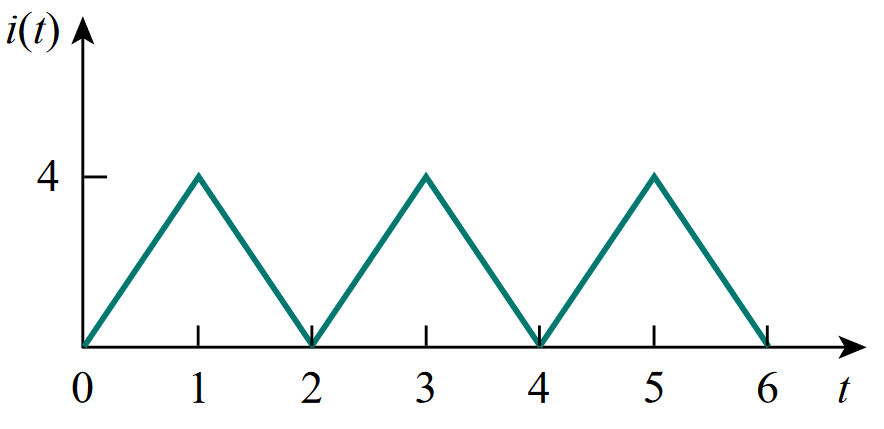
\includegraphics[width=0.4\textwidth]{Fig11.15_ElectricCircuit_SadikuPg446_3E}
			 \caption{}
             \label{fig:currentWaveform}
        \end{figure}
		
\begin{solution}

\end{solution}		
%%%%%%%%%%%%%%%%%%%%%%%%%%%%%%%%%%%%%%%%%%%%%%%%%%%%%%%%%%%			
\end{parts}

